\documentclass[11pt,a4paper]{article}
\usepackage[T1]{fontenc}
\usepackage[utf8]{inputenc}
\usepackage{lmodern}
\usepackage{microtype}
\usepackage[margin=2.6cm]{geometry}
\usepackage{setspace}
\usepackage{graphicx}
\usepackage{booktabs}
\usepackage{array}
\newcolumntype{L}[1]{>{\raggedright\arraybackslash}p{#1}}
\usepackage{threeparttable}
\usepackage[font=small,labelfont=bf]{caption}
\usepackage{float}
\usepackage{amsmath,amssymb}
\usepackage{enumitem}
\usepackage{xcolor}
\usepackage[authoryear,round]{natbib}
\usepackage{titlesec}
\usepackage{fancyhdr}
\usepackage[hidelinks]{hyperref}

\definecolor{edition}{gray}{0.94}
\setstretch{1.15}
\setlist{itemsep=2pt,topsep=4pt}
\titleformat{\section}{\large\bfseries}{\thesection}{0.8em}{}
\titleformat{\subsection}{\normalsize\bfseries}{\thesubsection}{0.8em}{}
\pagestyle{fancy}
\fancyhf{}
\fancyhead[L]{\small Simons --- Oil volatility and uncertainty, revised edition (2026)}
\fancyhead[R]{\small\thepage}
\renewcommand{\headrulewidth}{0.3pt}

\newcommand{\dln}{\Delta\ln}

\begin{document}

\begin{titlepage}
\centering
\vspace*{2.5cm}
{\small EDHEC Business School --- International BBA\par}
\vspace{1.8cm}
{\LARGE\bfseries Financial market \& oil volatility\\[4pt] within distressed economies\par}
\vspace{0.5cm}
{\large Wavelet coherence evidence from the early 21st century\par}
\vspace{1.2cm}
{\large\itshape Revised edition, 2026\par}
\vspace{2cm}
{\Large Yann Simons\par}
\vfill
\begin{minipage}{0.86\textwidth}
\small
Revised edition of the final thesis written for the EDHEC International BBA
(4th year, 2020/2021 programme; thesis director: Ms Stepanyan). The original
version, dated July 2022, is kept unchanged in the same repository
(\texttt{thesis/}). This edition keeps the research question, the data and the
sample of the original; it corrects the text and re-runs the empirical analysis.
All results reported here are produced by the script
\texttt{revised\_analysis.py} distributed with this document.
\end{minipage}
\vspace{1.5cm}
\end{titlepage}

\begin{abstract}
\noindent
This thesis asks how oil prices respond to geopolitical and economic uncertainty
during crises. Using monthly data for West Texas Intermediate (WTI) crude oil,
the Economic Policy Uncertainty index (EPU) of \citet{baker2016} and the
Geopolitical Risk index (GPR) of \citet{caldara2022} from January 2000 to March
2022, I combine classical time-series tools with bivariate wavelet coherence.
Oil prices are non-stationary in levels, so all models are estimated in log
changes. Rising economic policy uncertainty is associated with falling oil
prices: the contemporaneous elasticity is $-0.074$ (HAC $p=0.026$), and lagged
uncertainty adds a further negative effect, although uncertainty explains only a
small share of monthly oil-price variance. Geopolitical risk shows no significant
association with oil returns on average. Wavelet coherence locates the
EPU--oil link in crisis periods (2001--2004, 2007--2010, 2018--2021), mainly at
8--16-month horizons and in anti-phase; uncertainty leads oil during the
early-2000s and the global financial crisis, while oil leads during the
pandemic. Coherence between oil and geopolitical risk is weaker and confined to
2000--2004. Economic uncertainty, rather than geopolitical risk, is the more
consistent companion of oil-market stress over the sample.

\medskip\noindent
\textbf{Keywords:} oil price, economic policy uncertainty, geopolitical risk,
wavelet coherence, Granger causality.
\end{abstract}

\section*{About this edition}
\addcontentsline{toc}{section}{About this edition}

\noindent\colorbox{edition}{\begin{minipage}{0.97\textwidth}\small
\vspace{4pt}
\textbf{What has not changed.} The research question, the three variables, the
data (same workbook, January 2000 -- March 2022) and the overall approach ---
classical econometrics first, wavelet coherence second.

\smallskip
\textbf{What has changed.}
(i) The text has been rewritten for clarity and corrected where it contained
factual or statistical errors (see the erratum below).
(ii) The empirical analysis has been re-run in Python on the identical data,
with a complete unit-root battery (ADF, Phillips--Perron, KPSS), models in log
changes with heteroskedasticity- and autocorrelation-robust standard errors,
Granger tests in both directions with information-criterion lag selection,
rolling correlations, and wavelet coherence with Monte Carlo significance,
cone of influence and phase (lead--lag) analysis.
(iii) Section~\ref{sec:compare} compares the 2022 and 2026 conclusions point by point.
\vspace{4pt}
\end{minipage}}

\subsection*{Erratum to the 2022 edition}

\begin{small}
\begin{tabular}{@{}L{0.47\textwidth}L{0.49\textwidth}@{}}
\toprule
2022 edition & Correction \\
\midrule
The Granger tests are ``significant enough to be relevant at the 5\% threshold''. &
None is: $p=0.156$ (EPU$\to$WTI), $0.192$ (GPR$\to$WTI), $0.311$ (WTI$\to$GPR). \\[2pt]
``Multiple p-values would meet significance level'' (regressions). &
In the 2022 regression no coefficient was significant at 5\% (EPU: $p=0.086$). \\[2pt]
GPR described with the EPU methodology (``index of news articles discussing
economic policy uncertainty''). &
GPR measures the share of newspaper articles about adverse geopolitical events
and threats \citep{caldara2022}. \\[2pt]
OPEC members listed include Ecuador and Qatar; Congo and Equatorial Guinea omitted. &
In 2022 OPEC had 13 members; Qatar left in 2019 and Ecuador in 2020. \\[2pt]
The United States is ``the largest oil importer''. &
The United States is the largest producer; China has been the largest crude-oil
importer since 2017. \\[2pt]
``The wavelet approach lacks directional indications.'' &
The phase of the cross-wavelet transform indicates in-/anti-phase movement and
which series leads; it is used in Section~\ref{sec:wavelet}. \\[2pt]
Footnote: ``negative skewness with right tail''. &
Negative skewness means a longer \emph{left} tail. \\[2pt]
Stationarity assessed with Phillips--Perron only, on returns. &
Levels and changes are tested with three tests; WTI is non-stationary in levels
(Table~\ref{tab:unitroot}). \\
\bottomrule
\end{tabular}
\end{small}

\bigskip
{\setcounter{tocdepth}{1}\small\tableofcontents}
\newpage

\section{Introduction}

Globalisation and free-market theory promise low-friction trade in goods and
services, yet the early twenty-first century has repeatedly shown the limits of
that model for energy. Oil is traded to secure a continuous physical supply, but
the market also carries financial risks that tend to materialise precisely when
economies are under stress. Over two decades the price of a barrel of WTI has
moved from below US\$20 to above US\$130, and in April 2020 the front-month
futures contract even settled below zero.

This thesis asks a simple question: \emph{how is the oil price affected by
geopolitical and economic uncertainty during crises since 2000?} I measure the
two sources of uncertainty with newspaper-based indices --- the Economic Policy
Uncertainty index (EPU) and the Geopolitical Risk index (GPR) --- and relate them
to the WTI price. The aim is twofold: to quantify the association between
uncertainty and oil prices, and to identify \emph{when} and at \emph{which
horizons} the two move together. The second aim motivates the use of wavelet
coherence, which, unlike a single regression coefficient, shows how a
relationship evolves across time and frequencies.

The answer matters beyond financial markets. Oil prices feed into transport,
heating and the price of most goods, so their volatility is a direct cost for
households and firms, and a recurrent concern for policymakers. A clearer view of
which kind of uncertainty accompanies oil-market stress, and with what timing, is
useful for anyone exposed to energy prices.

The thesis proceeds as follows. Section~\ref{sec:market} recalls the main actors
and crises of the oil market since 2000. Section~\ref{sec:uncertainty} discusses
why uncertainty should matter for oil prices and reviews the relevant
literature. Section~\ref{sec:hyp} states the hypotheses. Sections~\ref{sec:data}
and~\ref{sec:method} present the data and methods, Section~\ref{sec:results} the
results, Section~\ref{sec:compare} compares them with the 2022 edition, and
Section~\ref{sec:conclusion} concludes.

\section{The oil market in the twenty-first century}\label{sec:market}

\subsection{Main actors}

The Organization of the Petroleum Exporting Countries (OPEC), founded in 1960,
coordinates the petroleum policies of its members --- thirteen countries in 2022,
including Saudi Arabia, Iraq, Iran, the United Arab Emirates, Kuwait, Venezuela
and Nigeria. Its main instruments are production quotas, decided at ministerial
meetings, and the OPEC Reference Basket price, which tracks the crudes its members
produce. Since 2016 OPEC has also coordinated output with a group of non-member
producers led by Russia (``OPEC+'').

The United States is the other pivotal actor. It became the world's largest
crude-oil producer in 2018 on the back of the shale revolution, while remaining a
major importer; China has been the largest crude importer since 2017. The
International Energy Agency (IEA), created in 1974 after the 1973 embargo decided
by Arab producers during the Yom Kippur War, coordinates the energy policies and
emergency stocks of consuming countries. The 2022 confrontation between Russia
and Western countries over Ukraine revived exactly the type of supply risk the
IEA was designed to manage.

\subsection{Crises and price swings since 2000}

The sample covers a sequence of distinct shocks:
\begin{itemize}
\item \textbf{2001--2003}: the 11 September attacks, the war in Afghanistan and the
run-up to the 2003 invasion of Iraq, a period of exceptionally high geopolitical
risk;
\item \textbf{2007--2009}: the global financial crisis. Oil rose to a record of
about US\$134 per barrel in mid-2008 (monthly average) before collapsing as
demand fell and credit tightened;
\item \textbf{2010--2013}: the Arab Spring and the Libyan and Syrian conflicts,
which raised fears of supply disruptions in the Middle East and North Africa;
\item \textbf{2014--2016}: the price collapse driven by booming US shale output
and OPEC's decision in late 2014 not to cut production, alongside the first
Russia--Ukraine crisis;
\item \textbf{2020}: the Covid-19 pandemic. Lockdowns cut demand abruptly,
storage filled up, and WTI futures briefly traded at negative prices;
\item \textbf{2022}: Russia's invasion of Ukraine, a supply shock that pushed
prices back above US\$100.
\end{itemize}

Across these episodes the same fundamental drivers recur: production costs and
spare capacity, global demand and economic growth, inventories, and political
events in producing regions. What differs from one crisis to another is whether
the shock originates in demand (2008, 2020) or in supply and politics (2003,
2011, 2022) --- a distinction emphasised by \citet{kilian2009}.

\section{Uncertainty and oil prices}\label{sec:uncertainty}

\subsection{Why uncertainty should matter}

Oil is unusual among financial assets: it is consumed globally, it is a large
input in household budgets --- transport accounts for roughly two-thirds of US
petroleum use --- and its supply is concentrated in politically sensitive
regions. Uncertainty can therefore move oil prices through two channels that
work in opposite directions. \emph{Economic} uncertainty depresses investment,
consumption and trade, and hence the demand for oil; it should be associated
with lower prices. \emph{Geopolitical} risk threatens supply and raises
precautionary demand; it should be associated with higher prices, at least
initially. Speculative positioning in oil futures can amplify both effects.

\subsection{Measuring uncertainty}

\citet{baker2016} build the EPU index from the frequency of newspaper articles
containing terms about the economy, policy and uncertainty in major US
newspapers. \citet{caldara2022} build the GPR index from the share of articles
in leading newspapers that discuss adverse geopolitical events and threats ---
wars, terrorist attacks, military tensions. Both indices are monthly, available
from 2000 and widely used in the energy literature.

\subsection{Related literature}

Since \citet{hamilton1983}, a large literature has documented the links between
oil prices and the macroeconomy, and \citet{kilian2009} showed that the effect of
an oil price change depends on the shock behind it. \citet{antonakakis2014} document
time-varying spillovers between oil price shocks and economic policy
uncertainty. Wavelet methods have become
popular in this field because they separate short- and long-run co-movements:
\citet{sharif2020} use them to study oil, stock markets, geopolitical risk and
policy uncertainty during Covid-19, and \citet{wang2022} combine wavelet
coherence with a quantile causality test and find that both geopolitical risk
and economic policy uncertainty affect oil price fluctuations, especially after
2016. \citet{bourghelle2021} document the specific volatility dynamics of oil
during the pandemic. This thesis applies the same tools to the joint
EPU--GPR--WTI system over 2000--2022, and pays particular attention to
statistical significance and to the direction of the co-movements.

\section{Hypotheses}\label{sec:hyp}

Following the discussion above, the predictions are:
\begin{description}[leftmargin=1.2cm,style=nextline]
\item[H1] Economic policy uncertainty is negatively associated with oil price
changes, through lower expected demand.
\item[H2] Geopolitical risk is positively associated with oil price changes,
through supply fears and precautionary demand.
\item[H3] The co-movements between uncertainty and oil are concentrated in
crisis periods rather than spread evenly over the sample.
\end{description}

\section{Data}\label{sec:data}

The sample consists of monthly observations from January 2000 to March 2022
(267 months): the WTI spot price (FRED, Federal Reserve Bank of St.\ Louis), the
US EPU index (policyuncertainty.com) and the GPR index (matteoiacoviello.com).
Figure~\ref{fig:series} plots the three series with the main crisis periods
shaded.

\begin{figure}[!tb]
\centering
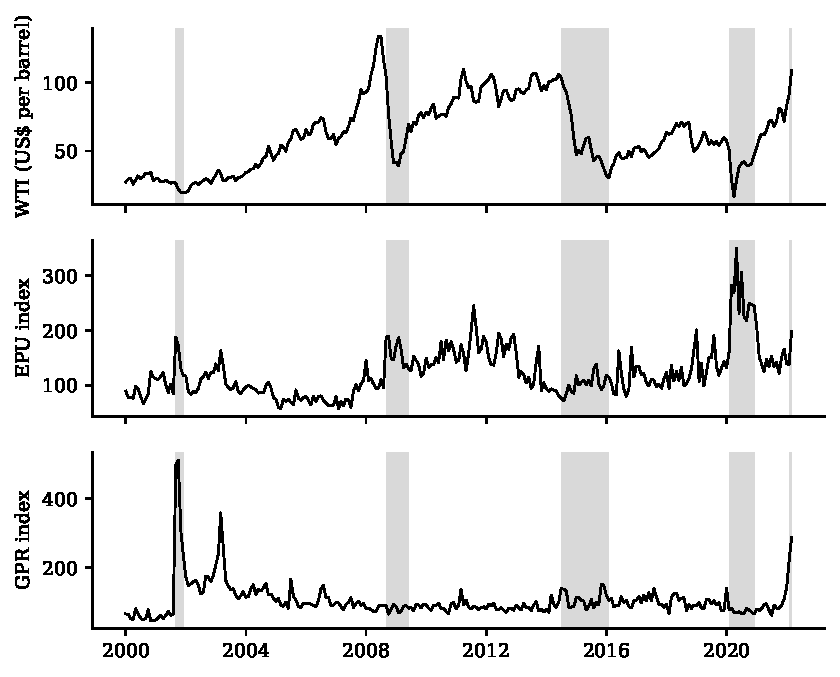
\includegraphics[width=\textwidth]{fig/fig1_series.pdf}
\caption{WTI, EPU and GPR, January 2000 -- March 2022. Shaded: September--December
2001, the 2008--09 financial crisis, the 2014--16 oil price collapse, 2020 and
February--March 2022.}
\label{fig:series}
\end{figure}

Table~\ref{tab:desc} reports descriptive statistics for the levels and for the
monthly log changes, $\dln X_t = \ln X_t - \ln X_{t-1}$, which are used in all
models. The 2022 edition used simple percentage changes; log changes are less
affected by the extreme spikes of the GPR index (its simple monthly change
reaches $+678\%$ in September 2001). All series are far from normal: the
Jarque--Bera test rejects normality everywhere, oil changes are negatively skewed
with a kurtosis above 10, and GPR changes are dominated by a few very large
positive jumps.

\begin{table}[H]
\centering
\caption{Descriptive statistics}
\label{tab:desc}
\begin{small}
\begin{tabular}{lrrrrrr}
\toprule
 & WTI & EPU & GPR & $\Delta\ln$WTI & $\Delta\ln$EPU & $\Delta\ln$GPR \\
\midrule
Mean & 61.393 & 123.038 & 103.697 & 0.0052 & 0.0030 & 0.0056 \\
Median & 59.000 & 111.886 & 90.652 & 0.017 & -0.015 & -0.0020 \\
Std. dev. & 25.683 & 45.355 & 52.743 & 0.106 & 0.192 & 0.231 \\
Min & 16.550 & 57.203 & 45.061 & -0.568 & -0.643 & -0.600 \\
Max & 133.880 & 350.460 & 512.530 & 0.546 & 0.803 & 2.051 \\
Skewness & 0.386 & 1.458 & 4.410 & -0.974 & 0.486 & 2.731 \\
Kurtosis & 2.318 & 6.302 & 29.833 & 10.747 & 5.187 & 25.402 \\
Jarque-Bera & 11.8 & 215.9 & 8,876 & 707.3 & 63.5 & 5,893 \\
JB p-value & 0.0027 & <0.001 & <0.001 & <0.001 & <0.001 & <0.001 \\
\bottomrule
\end{tabular}

\end{small}
\par\smallskip\parbox{0.92\textwidth}{\footnotesize Levels: 267 observations;
log changes: 266. Kurtosis is not excess kurtosis (3 for a normal
distribution).}
\end{table}

\section{Methodology}\label{sec:method}

\paragraph{Stationarity.} Each series is tested in levels and in log changes with
the augmented Dickey--Fuller test \citep{dickey1979} and the Phillips--Perron
test \citep{phillips1988}, whose null hypothesis is a unit root, and with the
KPSS test \citep{kpss1992}, whose null is stationarity. Using tests with opposite
nulls guards against the low power of any single test.

\paragraph{Regressions.} I estimate
\begin{equation}
\dln \text{WTI}_t = \alpha + \beta_E\, \dln \text{EPU}_t + \beta_G\, \dln \text{GPR}_t + \varepsilon_t ,
\end{equation}
with Newey--West standard errors \citep{newey1987} robust to
heteroskedasticity and autocorrelation (6 lags), and a dynamic version adding
one lag of each variable. For comparison, the 2022 specification (simple
percentage changes, classical standard errors) is reproduced.

\paragraph{Granger causality.} For each pair, a bivariate VAR in log changes is
estimated with the lag length chosen by the Akaike (AIC) and Bayesian (BIC)
information criteria (maximum 12 lags), and I test whether the lags of one
variable improve the forecast of the other \citep{granger1969}, in both
directions.

\paragraph{Wavelet coherence.}\label{sec:wavelet} The continuous wavelet
transform decomposes a series into time and frequency (period) components
\citep{torrence1998}. For two series $x$ and $y$ with transforms $W^x$ and $W^y$,
the wavelet coherence
\begin{equation}
R^2(s,t)=\frac{\left|S\!\left(s^{-1}W^{xy}(s,t)\right)\right|^2}
{S\!\left(s^{-1}|W^{x}(s,t)|^2\right)\,S\!\left(s^{-1}|W^{y}(s,t)|^2\right)},
\qquad W^{xy}=W^{x}\,\overline{W^{y}},
\end{equation}
where $S$ is a smoothing operator, behaves like a local squared correlation
between 0 and 1 at each time $t$ and period $s$ \citep{grinsted2004}. I use the
Morlet wavelet on periods from 2 to 64 months. Significance at the 5\% level is
assessed by Monte Carlo simulation against red-noise (AR(1)) benchmarks, and
results outside the cone of influence, where edge effects distort the transform,
are not interpreted. The phase angle $\phi$ of the smoothed cross-wavelet
transform tells how the two series move: $|\phi|<\pi/2$ means in phase (same
direction), $|\phi|>\pi/2$ anti-phase (opposite directions); within each case, the
sign of $\phi$ indicates which series leads \citep{aguiar2014}. In the figures,
arrows pointing right indicate in-phase movement and arrows pointing left
anti-phase movement.

\section{Results}\label{sec:results}

\subsection{Stationarity}

Table~\ref{tab:unitroot} confirms that the WTI price is non-stationary in levels:
neither ADF ($p=0.19$) nor Phillips--Perron ($p=0.28$) rejects a unit root, and
KPSS rejects stationarity ($p<0.01$). Evidence for the EPU level is mixed, while
the GPR level is stationary --- it is an index that reverts after each spike. All
log changes are clearly stationary. Regressions in levels would therefore risk
being spurious, which is why every model below uses log changes.

\begin{table}[H]
\centering
\caption{Unit-root and stationarity tests}
\label{tab:unitroot}
\begin{small}
\begin{tabular}{lrrrrrr}
\toprule
 & \multicolumn{2}{c}{ADF} & \multicolumn{2}{c}{Phillips-Perron} & \multicolumn{2}{c}{KPSS} \\
\cmidrule(lr){2-3}\cmidrule(lr){4-5}\cmidrule(lr){6-7}
Series & stat. & $p$ & stat. & $p$ & stat. & $p$ \\
\midrule
$\ln$ WTI & -2.24 & 0.192 & -2.02 & 0.277 & 0.785 & 0.008 \\
$\ln$ EPU & -2.44 & 0.132 & -4.99 & 0.000 & 0.779 & 0.008 \\
$\ln$ GPR & -5.35 & 0.000 & -5.47 & 0.000 & 0.221 & 0.231 \\
$\Delta\ln$ WTI & -11.06 & 0.000 & -11.77 & 0.000 & 0.057 & 0.835 \\
$\Delta\ln$ EPU & -11.58 & 0.000 & -26.89 & 0.000 & 0.079 & 0.700 \\
$\Delta\ln$ GPR & -7.35 & 0.000 & -22.26 & 0.000 & 0.107 & 0.554 \\
\bottomrule
\end{tabular}

\end{small}
\par\smallskip\parbox{0.92\textwidth}{\footnotesize ADF (lag length by AIC) and
Phillips--Perron: null of a unit root. KPSS: null of stationarity. All tests
include a constant.}
\end{table}

\subsection{Regressions}

Table~\ref{tab:ols} reports the regressions. Column (1) reproduces the 2022
specification: on the 266 available monthly changes, the EPU coefficient is
$-0.065$ ($p=0.043$); the 2022 run, on a slightly different version of the
workbook, reported $-0.054$ ($p=0.086$). Column (2) is the revised specification:
a 1\% increase in economic policy uncertainty is associated with a 0.074\%
fall in the oil price in the same month, significant at 5\% with robust standard
errors ($p=0.026$). Geopolitical risk has no significant effect
($\beta_G=0.020$, $p=0.27$).

Column (3) adds lags. The contemporaneous EPU effect remains ($-0.085$,
$p=0.016$) and is reinforced by a negative effect of the previous month's
uncertainty ($-0.094$, $p=0.049$), while oil changes show positive momentum from
one month to the next ($0.23$, $p<0.01$). The explanatory power remains modest
($R^2=0.11$, of which only about 2 points come from contemporaneous
uncertainty): uncertainty is a statistically robust but economically small
companion of monthly oil price changes. H1 is supported; H2 is not.

\begin{table}[H]
\centering
\caption{Oil price changes and uncertainty}
\label{tab:ols}
\begin{small}
\begin{tabular}{lccc}
\toprule
 & (1) 2022 specification & (2) Revised & (3) Revised, lags \\
 & simple \% changes, OLS SE & log changes, HAC SE & log changes, HAC SE \\
\midrule
Constant & $0.0119^{*}$ & $0.0053$ & $0.0042$ \\
 & $(0.0064)$ & $(0.0068)$ & $(0.0055)$ \\
EPU change & $-0.0647^{**}$ & $-0.0740^{**}$ & $-0.0845^{**}$ \\
 & $(0.0318)$ & $(0.0332)$ & $(0.0349)$ \\
GPR change & $0.0064$ & $0.0199$ & $0.0096$ \\
 & $(0.0145)$ & $(0.0182)$ & $(0.0196)$ \\
WTI change, $t-1$ &  &  & $0.2301^{***}$ \\
 &  &  & $(0.0890)$ \\
EPU change, $t-1$ &  &  & $-0.0939^{**}$ \\
 &  &  & $(0.0478)$ \\
GPR change, $t-1$ &  &  & $0.0114$ \\
 &  &  & $(0.0326)$ \\
\midrule
$R^2$ & 0.016 & 0.018 & 0.108 \\
Observations & 266 & 266 & 265 \\
\bottomrule
\end{tabular}

\end{small}
\par\smallskip\parbox{0.92\textwidth}{\footnotesize Dependent variable: monthly
change in WTI. Column (1): simple percentage changes and classical standard
errors, as in 2022. Columns (2)--(3): log changes, Newey--West standard errors
(6 lags). Standard errors in parentheses; $^{*}$, $^{**}$, $^{***}$: significance
at 10\%, 5\%, 1\%.}
\end{table}

\subsection{Granger causality}

Table~\ref{tab:granger} reports the Granger tests. The AIC selects three lags
for every pair, as in 2022, and the BIC one lag. Uncertainty helps forecast oil
only weakly: EPU Granger-causes WTI at 5\% with one lag ($p=0.035$) but not with
three ($p=0.135$), and GPR never does. In the other direction, oil price changes
help forecast EPU at the margin ($p=0.049$ with three lags, $0.066$ with one),
which is consistent with oil shocks feeding economic uncertainty. Oil does not
Granger-cause GPR at 5\%. The 2022 tests are reproduced closely on the original
simple changes ($p=0.145$, $0.176$ and $0.304$ for the three tests reported
then); none of them was significant.

\begin{table}[H]
\centering
\caption{Granger causality tests (log changes)}
\label{tab:granger}
\begin{small}
\begin{tabular}{lcccc}
\toprule
 & \multicolumn{2}{c}{Lag selected by AIC} & \multicolumn{2}{c}{Lag selected by BIC} \\
\cmidrule(lr){2-3}\cmidrule(lr){4-5}
Null hypothesis & lag, $F$ & $p$ & lag, $F$ & $p$ \\
\midrule
EPU $\nrightarrow$ WTI & 3, 1.87 & 0.135 & 1, 4.52 & 0.035 \\
GPR $\nrightarrow$ WTI & 3, 1.93 & 0.125 & 1, 0.01 & 0.932 \\
WTI $\nrightarrow$ EPU & 3, 2.66 & 0.049 & 1, 3.41 & 0.066 \\
WTI $\nrightarrow$ GPR & 3, 0.98 & 0.402 & 1, 3.21 & 0.074 \\
\bottomrule
\end{tabular}

\end{small}
\par\smallskip\parbox{0.92\textwidth}{\footnotesize $X \nrightarrow Y$: null
hypothesis that $X$ does not Granger-cause $Y$. $F$-tests from bivariate VARs;
maximum lag 12.}
\end{table}

\subsection{Time-varying correlation}

Before turning to wavelets, Figure~\ref{fig:rolling} shows 36-month rolling
correlations. The WTI--EPU correlation is negative on average ($-0.10$) and
reaches its most negative value ($-0.46$) in the window ending in March 2020,
when the pandemic hit both series at once. The WTI--GPR correlation fluctuates
around zero (average $0.02$), with a positive peak ($0.36$) in the window ending
in October 2008. A single full-sample coefficient ($-0.13$ for EPU, $0.02$ for
GPR) therefore hides substantial variation over time.

\begin{figure}[htbp]
\centering
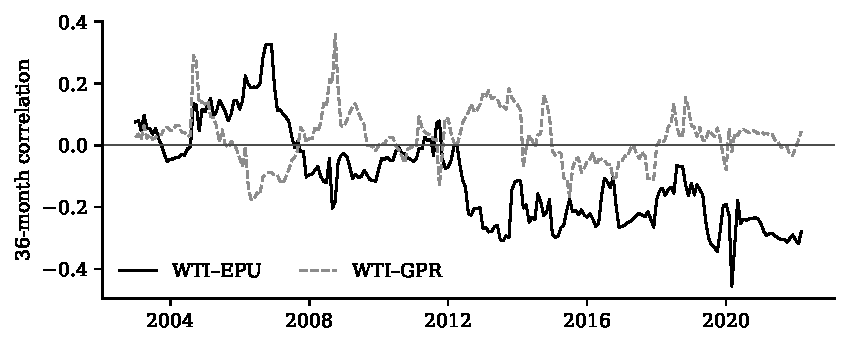
\includegraphics[width=\textwidth]{fig/fig4_rolling.pdf}
\caption{36-month rolling correlation between monthly log changes of WTI and of EPU (solid) and GPR (dashed).}
\label{fig:rolling}
\end{figure}

\subsection{Wavelet coherence}

Figures~\ref{fig:wtcepu} and~\ref{fig:wtcgpr} show the wavelet coherence between
oil price changes and changes in each uncertainty index. Darker areas indicate
higher coherence; thick contours enclose regions significant at 5\%; the hatched
area lies outside the cone of influence.

\begin{figure}[htbp]
\centering
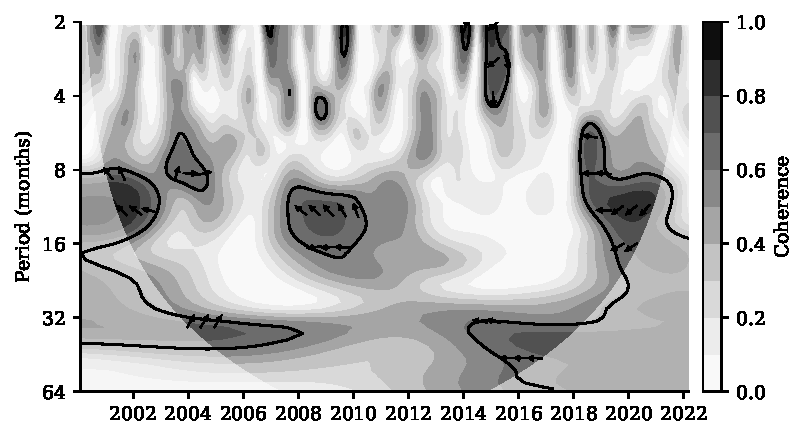
\includegraphics[width=\textwidth]{fig/fig2_wtc_epu.pdf}
\caption{Wavelet coherence between WTI and EPU (monthly log changes). Arrows
are shown in significant regions: right = in phase, left = anti-phase.}
\label{fig:wtcepu}
\end{figure}

\paragraph{Oil and economic policy uncertainty.} Significant coherence covers
11.5\% of the time--frequency plane inside the cone of influence --- more than
twice the share expected under the null of no relationship. It is concentrated
at 8--16-month periods (26\% of that band is significant) and, to a lesser
extent, at 32--64 months (24\%), and it appears in three crisis episodes:
\begin{itemize}
\item \textbf{2001--2004} (8--16 months): anti-phase, with uncertainty leading
oil --- rising uncertainty after the 2001 recession and 11 September is followed
by weaker oil prices;
\item \textbf{2007--2010} (8--16 months): the strongest and most coherent island,
again anti-phase with uncertainty leading in nearly 90\% of significant cells ---
the financial crisis raised uncertainty first and depressed oil demand
afterwards;
\item \textbf{2018--2021} (8--32 months): anti-phase, but with oil leading in
about 80\% of significant cells --- during the pandemic the collapse in oil
demand and prices accompanied, and partly preceded, the surge in uncertainty.
\end{itemize}
Across all significant cells, 77\% are in anti-phase, which matches the negative
regression coefficients. At long horizons (32--64 months) the coherence of the
mid-2000s and of 2014--2018 lies close to the edge of the cone of influence and
should be read with caution.

\begin{figure}[htbp]
\centering
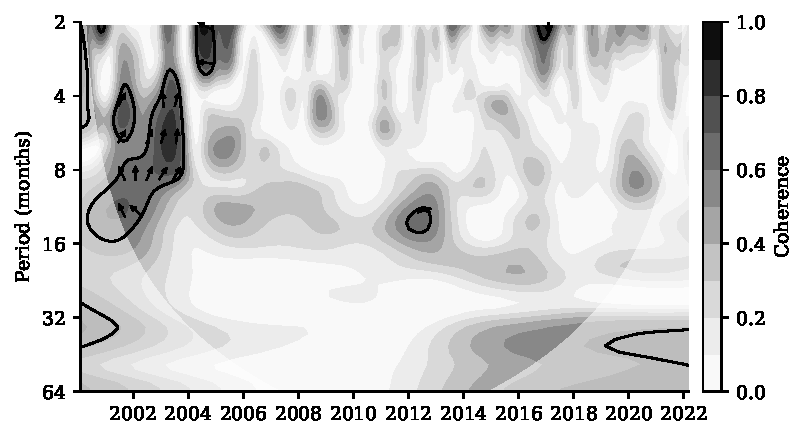
\includegraphics[width=\textwidth]{fig/fig3_wtc_gpr.pdf}
\caption{Wavelet coherence between WTI and GPR (monthly log changes).}
\label{fig:wtcgpr}
\end{figure}

\paragraph{Oil and geopolitical risk.} Coherence with geopolitical risk is much
weaker: only 4.1\% of the plane is significant, roughly what chance alone would
produce. The one substantial region covers 2000--2004 at periods of 2--16
months, the period of 11 September, the war in Afghanistan and the run-up to the
Iraq war; within it, a third of the 2001--2002 window is significant. The phase
there is close to $90^\circ$: the two series move with about a quarter-cycle
shift rather than strictly together or apart. At 2--8 months oil tends to move
first (about 70\% of significant cells), whereas at 8--16 months geopolitical
risk tends to lead, so the direction of the link is not clear-cut. A small island appears
around 2012 at about one year (the Arab Spring and the Libyan and Syrian
conflicts). No significant coherence is found in 2008--2009, 2014--2016 or
2020--2022.

H3 is therefore supported for economic policy uncertainty, whose link with oil
is concentrated in crises, and only partially for geopolitical risk, whose link
is confined to the early 2000s.

\section{Comparison with the 2022 edition}\label{sec:compare}

\begin{small}
\begin{tabular}{@{}L{0.24\textwidth}L{0.33\textwidth}L{0.37\textwidth}@{}}
\toprule
Point & 2022 edition & Revised analysis (2026) \\
\midrule
Regression of oil on EPU and GPR & ``Not robust enough'' to draw conclusions &
EPU negative and significant at 5\% with robust errors; GPR not significant;
low explanatory power \\[2pt]
Granger causality & Described as significant at 5\% (they were not) &
Weak: EPU$\to$WTI only with one lag; marginal feedback WTI$\to$EPU; nothing for GPR \\[2pt]
EPU coherence & 2001--2005, 2008 cluster, 2016, Covid period &
Confirmed for 2001--2004, 2007--2010 and 2018--2021; 2016 visible only at long
horizons near the cone edge \\[2pt]
GPR coherence & After 2001, around 2004, and after Covid &
Confirmed for 2000--2004 (plus a small island around 2012); no significant post-Covid coherence \\[2pt]
Common horizon & ``8-to-10-month level'' for both &
8--16 months for EPU in all three crises; for GPR only in 2001--2004 \\[2pt]
Direction & Not identifiable with wavelets &
Mostly anti-phase for EPU; uncertainty leads in 2001--04 and 2007--10, oil leads in 2020 \\[2pt]
Main message & Economic uncertainty matters more than geopolitical risk &
Confirmed, and now supported by significance tests \\
\bottomrule
\end{tabular}
\end{small}

\medskip
The core intuition of the 2022 thesis survives: economic policy uncertainty, more
than geopolitical risk, accompanies oil-market stress, and it does so mainly
during crises. What changes is the strength of the evidence and its precision.
The regression evidence is stronger than the original text concluded, once the
model is estimated in log changes with appropriate standard errors; the Granger
evidence is weaker than the original text stated; and the wavelet evidence for
geopolitical risk is narrower than the 2022 reading of the figures suggested.

\section{Conclusion}\label{sec:conclusion}

This thesis set out to understand how economic and geopolitical uncertainty
relate to oil prices in crisis times. Over 2000--2022, rising economic policy
uncertainty is associated with falling oil prices, contemporaneously and with a
one-month lag, and the association is concentrated in the early-2000s
slowdown, the global financial crisis and the pandemic, at horizons of roughly
one year. The timing differs by crisis: uncertainty led oil in 2001--2004 and
2007--2010, whereas oil led during the pandemic, when a demand collapse hit
prices directly. Geopolitical risk, despite its prominence in the media, has no
average effect on monthly oil returns and a significant co-movement only in the
2001--2003 sequence of attacks and wars.

Three limits frame these findings. First, uncertainty explains a small share of
monthly oil price changes; supply decisions, inventories and global demand
remain the main drivers. Second, wavelet coherence and Granger tests describe
co-movement and predictability, not structural causality. Third, the sample ends
in March 2022, at the start of the war in Ukraine. Natural extensions are to
extend the sample, to add macroeconomic controls such as inflation and industrial
production, to compare WTI with Brent, and to study the tails of the oil return
distribution with quantile methods, as in \citet{wang2022}.

\section*{Reproducibility}
\addcontentsline{toc}{section}{Reproducibility}

All tables and figures are produced by \texttt{revised\_analysis.py} (Python 3,
with pandas, statsmodels, arch, scipy, pycwt and matplotlib) from
\texttt{data/thesis\_dataset\_with\_returns.csv}. The Monte Carlo significance
of the wavelet coherence uses a fixed random seed, so the results are exactly
reproducible.

\begin{thebibliography}{99}
\setlength{\itemsep}{1pt}\small

\bibitem[Aguiar-Conraria and Soares(2014)]{aguiar2014}
Aguiar-Conraria, L. and Soares, M. J. (2014). The continuous wavelet transform:
moving beyond uni- and bivariate analysis. \emph{Journal of Economic Surveys},
28(2), 344--375.

\bibitem[Antonakakis et~al.(2014)]{antonakakis2014}
Antonakakis, N., Chatziantoniou, I. and Filis, G. (2014). Dynamic spillovers of
oil price shocks and economic policy uncertainty. \emph{Energy Economics}, 44,
433--447.

\bibitem[Baker et~al.(2016)]{baker2016}
Baker, S. R., Bloom, N. and Davis, S. J. (2016). Measuring economic policy
uncertainty. \emph{Quarterly Journal of Economics}, 131(4), 1593--1636.

\bibitem[Bourghelle et~al.(2021)]{bourghelle2021}
Bourghelle, D., Jawadi, F. and Rozin, P. (2021). Oil price volatility in the
context of Covid-19. \emph{International Economics}, 167, 39--49.

\bibitem[Caldara and Iacoviello(2022)]{caldara2022}
Caldara, D. and Iacoviello, M. (2022). Measuring geopolitical risk.
\emph{American Economic Review}, 112(4), 1194--1225.

\bibitem[Dickey and Fuller(1979)]{dickey1979}
Dickey, D. A. and Fuller, W. A. (1979). Distribution of the estimators for
autoregressive time series with a unit root. \emph{Journal of the American
Statistical Association}, 74(366), 427--431.

\bibitem[Granger(1969)]{granger1969}
Granger, C. W. J. (1969). Investigating causal relations by econometric models
and cross-spectral methods. \emph{Econometrica}, 37(3), 424--438.

\bibitem[Grinsted et~al.(2004)]{grinsted2004}
Grinsted, A., Moore, J. C. and Jevrejeva, S. (2004). Application of the cross
wavelet transform and wavelet coherence to geophysical time series.
\emph{Nonlinear Processes in Geophysics}, 11, 561--566.

\bibitem[Hamilton(1983)]{hamilton1983}
Hamilton, J. D. (1983). Oil and the macroeconomy since World War II.
\emph{Journal of Political Economy}, 91(2), 228--248.

\bibitem[Kilian(2009)]{kilian2009}
Kilian, L. (2009). Not all oil price shocks are alike: disentangling demand and
supply shocks in the crude oil market. \emph{American Economic Review}, 99(3),
1053--1069.

\bibitem[Kwiatkowski et~al.(1992)]{kpss1992}
Kwiatkowski, D., Phillips, P. C. B., Schmidt, P. and Shin, Y. (1992). Testing
the null hypothesis of stationarity against the alternative of a unit root.
\emph{Journal of Econometrics}, 54(1--3), 159--178.

\bibitem[Newey and West(1987)]{newey1987}
Newey, W. K. and West, K. D. (1987). A simple, positive semi-definite,
heteroskedasticity and autocorrelation consistent covariance matrix.
\emph{Econometrica}, 55(3), 703--708.

\bibitem[Phillips and Perron(1988)]{phillips1988}
Phillips, P. C. B. and Perron, P. (1988). Testing for a unit root in time series
regression. \emph{Biometrika}, 75(2), 335--346.

\bibitem[Sharif et~al.(2020)]{sharif2020}
Sharif, A., Aloui, C. and Yarovaya, L. (2020). COVID-19 pandemic, oil prices,
stock market, geopolitical risk and policy uncertainty nexus in the US economy:
fresh evidence from the wavelet-based approach. \emph{International Review of
Financial Analysis}, 70, 101496.

\bibitem[Torrence and Compo(1998)]{torrence1998}
Torrence, C. and Compo, G. P. (1998). A practical guide to wavelet analysis.
\emph{Bulletin of the American Meteorological Society}, 79(1), 61--78.

\bibitem[Wang et~al.(2022)]{wang2022}
Wang, Y., Wei, M., Bashir, U. and Zhou, C. (2022). Geopolitical risk, economic
policy uncertainty and global oil price volatility --- an empirical study based
on quantile causality nonparametric test and wavelet coherence. \emph{Energy
Strategy Reviews}, 41, 100851.

\end{thebibliography}

\subsection*{Other sources cited in the 2022 edition}
{\small
\begin{itemize}[leftmargin=*]
\item Bekiros, S. D. and Diks, C. G. H. (2008). The relationship between crude oil
spot and futures prices: cointegration, linear and nonlinear causality.
\emph{Energy Economics}, 30(5), 2673--2685.
\item Blomberg, S. B., Hess, G. D. and Orphanides, A. (2004). The macroeconomic
consequences of terrorism. \emph{Journal of Monetary Economics}, 51(5),
1007--1032.
\item \emph{Do tense geopolitical factors drive crude oil prices?} Energies,
13(16), 4277 (2020).
\item \emph{Are geopolitical threats powerful enough to predict global oil price
volatility?} Environmental Science and Pollution Research (2021).
\item \emph{The impact of extreme events on energy price risk.} Energy Economics
(2021).
\item \emph{Impact of financial instability on international crude oil
volatility: new sight from a regime-switching framework.} Resources Policy (2022).
\item \emph{The economic costs of the Russia--Ukraine conflict.} NIESR Policy
Paper 32 (2022).
\item \emph{Evaluating a year of oil price volatility.} Federal Reserve Bank of
Kansas City, Macro Bulletin.
\end{itemize}
}

\end{document}
